%%%%%%%%%%%%%%%%%%%%%%%%%%%%%%%%%%%%%%%%%%%%%%%%%%%%%%%%%%%%%%%%%%%%%%%%%%%%%%%%%%%%%%%%%%%%%%%%%%%%%%
%
%   Filename    : chapter_4.tex 
%
%   Description : This file will contain your Design and Implementation.
%                 
%%%%%%%%%%%%%%%%%%%%%%%%%%%%%%%%%%%%%%%%%%%%%%%%%%%%%%%%%%%%%%%%%%%%%%%%%%%%%%%%%%%%%%%%%%%%%%%%%%%%%%

\Section{Design and Implementation}
\label{sec:designimplementation}

This chapter discusses the design and implementation of the open-source tool to extract relations. It includes the architectural design, extraction rules and issues encountered during development.

\subsection{Corpus}
\label{sec:corpus}

The input corpus for this study is comprised of 30 children's stories. Each were encoded digitally and modified to remove dialogues. The raw version was retained and used with the modified stories. For this research, the 2 corpus are named \emph{RAW} and \emph{MODIFIED}. Overall, 60 stories were used to extract the relations. Shown in Table \ref{tab:storygroups} are the different story groups and their corresponding age groups. 

\begin{table}[ht]   %t means place on top, replace with b if you want to place at the bottom
\centering
\caption{Children's Story Groups} \vspace{0.25em}
\begin{tabular}{|p{4cm}|p{2cm}|p{3cm}|} \hline
Group Name & No. of Stories & Age Group \\ \hline
Topsy Tim					& 5 & 4-7 y.o. \\ \hline
Little Life Lessons			& 16 & 4-7 y.o. \\ \hline
Jumpstart					& 7 & 8-10 y.o. \\ \hline
Winnie the Pooh				& 2 & 8-10 y.o. \\ \hline
\end{tabular}
\label{tab:storygroups}
\end{table}

\subsubsection{Modifications}
\label{sec:modifications}

As mentioned, each children's story in the corpus were modified to clean the data of any inconsistencies. This section details the different modifications done on the corpora.

\subsubsection*{Dialogues}

Stories are mostly composed of dialogues which are conversational in nature. They are mostly informal, has incomplete thought and use colloquial words. A dialogue has different elements, namely:

\begin{itemize}
\item \textbf{Quotation marks} - punctuation that signal a character's spoken word. It also defines the end of a narration and the start of the speech.
\item \textbf{Speech} - these are the spoken words. 
\item \textbf{Speaker Attributions} - the combination of a verb and a speaker. This signals the character speaking and the manner a speech is spoken.
\end{itemize}

Each element will be handled differently depending on the type of modification. The objective of these modifications is to convert these dialogues into complete and coherent sentences in order to yield proper extractions. In order to illustrate the dialogue modifications, here is an unmodified excerpt from one of the stories already in the corpus entitled ``A Wild Weather Day".

\begin{verse}
\itshape
It was a wild and windy day. The JumpStart ship was headed for Tree Fort Island. \\
Frankie was at the wheel. The sails flapped in the wind. The ship raced through the water. \\
``Why are we going so fast?" Pierre asked. ``The wind is blowing us along on our adventure," CJ said. ``Did you know that wind is just air that is strong and fast?" \\
``Like Frankie!" Pierre said. ``He's strong and fast, too." \\
``Why is the sky getting so dark?" Pierre asked. \\
``I know why it's dark!" Eleanor said. ``Clouds get dark when they fill up with tiny drops of water." \\
``Look! They're almost the same color as your bow," Pierre said. \\
A big drop of rain fell on Pierre's nose. ``Oh, no!" he said. ``It's starting to rain!" \\
``The rain is coming from the clouds," CJ said. \\
``The water in the clouds got too heavy, and now it's falling down on us!" \\
``Just like when Hopsalot waters his garden," said Pierre. \\
\end{verse}

The first type of modification is done by transforming the dialogues into declarative sentences. Here is the modified version of the excerpt above:

\begin{verse}
\itshape
It was a wild and windy day. The JumpStart ship was headed for Tree Fort Island. \\
Frankie was at the wheel. The sails flapped in the wind. The ship raced through the water. \\
They are going so fast. The wind is blowing them along on their adventure. The wind is just air that is strong and fast. \\
Frankie is like the wind. He's strong and fast, too. \\
The sky is getting so dark.\\
Eleanor knows why it is dark. Clouds get dark when they fill up with tiny drops of water. \\
They are almost the same color as Eleanor's bow. \\
A big drop of rain fell on Pierre's nose. It is starting to rain! \\
The rain is coming from the clouds. \\
The water in the clouds got too heavy, and now it is falling down on them! \\
Just like when Hopsalot waters his garden. \\
\end{verse}

The second type is the usual transformation of direct to indirect speech. 

\begin{verse}
\itshape
It was a wild and windy day. The JumpStart ship was headed for Tree Fort Island. \\
Frankie was at the wheel. The sails flapped in the wind. The ship raced through the water. \\
Pierre asked why they were going so fast. CJ said that the wind was blowing them along on their adventure. He also asked if they know that wind is just air that is strong and fast. \\
Pierre said like Frankie. Pierre said that Frankie was strong and fast, too. \\
Pierre asked why the sky was getting so dark.\\
Eleanor said that she knew why it is dark. She explained that clouds get dark when they fill up with tiny drops of water.\\
Pierre said look! They are almost the same color as Eleanor's bow. \\
A big drop of rain fell on Pierre's nose. He was shocked. It is starting to rain. \\
CJ said that the rain is coming from the clouds. \\
The water in the clouds got too heavy, and now it is falling down on them. \\
Pierre said that it is just like when Hopsalot waters his garden. \\
\end{verse}
	
Through these examples, it is noticeable how one dialogue can be transformed two ways. In comparison, the first type of modification transforms dialogues into factual statements, sometimes even altering or removing the speaker attribution (verb and speaker). Here is a passage from the example:

\begin{verse}
\itshape
``Like Frankie!" Pierre said. ``He's strong and fast, too." \\
\end{verse}

The verb \textit{said} will be removed as well as the character (\textit{Pierre}) saying the dialogue. Since the focus is mostly on what is being said, and not who said it and the manner of saying, it was transformed into the following:

\begin{verse}
\itshape
Frankie is like the wind. He's strong and fast, too. \\
\end{verse}

On the other hand, the second type of modification usually retains the speaker attribution in its transformations. However, there can be changes in the verb used. Only one of these modifications are applied for each dialogue. The following rules were followed in transforming dialogues:

\begin{enumerate}
   \item For dialogues that are declarative in structure, the first type of modification is followed.
\begin{verse}
\itshape
\centering
``I know why it's dark!" Eleanor said. \\
to \\
Eleanor knows why it is dark. \\
\end{verse}
   \item For dialogues that are interrogative in structure and conveys a complete observation, action, or thought, the first type of modification is followed.
\begin{verse}
\itshape
\centering
``Why is the sky getting so dark?" Pierre asked. \\
to \\
The sky is getting so dark.\\
\end{verse}
   \item For dialogues that are interrogative in structure but has incomplete thought, action, or thought, the second type of modification is followed. These dialogues are usually follow up questions to previous statements made by other characters.
\begin{verse}
\itshape
\centering
``Why so?" Pierre asked. \\
to \\
Pierre asked why so.\\
\end{verse}
	\item For all dialogues transformed using the second type, the verb in the speaker attribute is changed to \textit{asked} or \textit{said}. Some examples include, \textit{whispered}, \textit{uttered} and \textit{mumbled}. This is done since these are just modifiers to how the dialogue was spoken. 
\end{enumerate}

After doing these modifications, it is important to note that the story has already changed. But in essence, the theme is still there. The intention was to make the actions and facts more apparent to the extraction tool. 

\subsubsection*{Interjections}

While modifying, there may be cases wherein a specific sentence or a line uttered by a character will be omitted or transformed into a declarative sentence not containing the original word/s. Such sentences can be interjections like ``Oh my!" and ``Alas!". These can be transformed as ``She was shocked" and ``He was concerned." The emotions conveyed by these interjections were used.

\subsubsection*{Contractions and Periods}

Aside from these, modifications such as removing contractions and periods (.) that do not actually mean the end of a sentence were done. With contractions, they were put back in their long form. For example, \textit{they'll} was transformed to \textit{they will}. This modification does not mean the tool used to extract the relations could not handle contractions. This just makes the results cleaner. It also disambiguates contractions from possessive nouns. For example, instances like \textit{Helen's} may mean ownership or just \textit{Helen is}. Removing nuances like these allows the tool to produce a more valid POS tagging and of course, extraction. 

As with the periods (.) like those found in titles (\textit{Mr.} and \textit{Dr.}), they were removed and the titles were transformed back into their long forms. For example, \textit{Mrs.} is transformed into \textit{Missus}. 

\subsubsection*{Non-English Words}

Lastly, story-specific modifications were done for the two \textit{Winnie the Pooh} stories. After careful examination, it was evident that the author was using non-existing English words in the dialogues of its characters. Words like \textit{suspicionated} and \textit{splendiferous} appeared in the story \textit{Everyone is special}. \textit{Tigger} is usually the character that uses such words due to his character trait. Such words were transformed to their actual English word counterparts. For example, \textit{suspicionated} and \textit{splendiferous} were transformed into \textit{suspected} and \textit{splendid}, respectively. This will make sure that all words are correctly tagged and the extracted relations contain valid concepts.

\subsection{Target Relations}
\label{sec:relations}

\begin{table}[H]   %t means place on top, replace with b if you want to place at the bottom
\centering
\caption{Target Relations} \vspace{0.25em}
\begin{tabular}{|p{3.5cm}|p{4cm}|p{5.5cm}|} \hline
\textbf{Element} & \textbf{Description} & \textbf{Example} \\ \hline
IsA					& Specifies what kind an entity is. & IsA(dog, pet) \\ \hline
PropertyOf			& Specifies an adjective to describe an entity. & PropertyOf(mango, yellow) \\ \hline
PartOf				& Specifies the \textit{parthood} of an entity in another entity. & PartOf(knob, door) \\ \hline
MadeOf				& Specifies a component of an entity. & MadeOf(door, wood) \\ \hline
CapableOf			& Specifies what an entity can do. & CapableOf(kid, jump) \\ \hline
OftenNear			& Specifies an entity near another entity in most instances. & OftenNear(chair, table) \\ \hline
LocationOf			& Specifies the location of an entity. & LocationOf(slide, play-ground) \\ \hline
UsedFor				& Specifies the use of an object in an activity. & UsedFor(toy, play) \\ \hline
EventForGoalEvent	& Represents an event that causes the fulfillment of a goal event. & EventForGoalEvent(go to playground, play football) \\ \hline
EventForGoalState	& Represents an event that causes the fulfillment of a goal state. & EventForGoalState(take a bath, be clean) \\ \hline
EffectOf			& Represents a cause-effect between two events. & EffectOf(skip breakfast, hungry) \\ \hline
EffectOfIsState		& Represents a cause-effect between an event and an end state. & EffectOfIsState(eat vegetables, health) \\ \hline
Happens				& Specifies the time an event/state happens. & Happens(breakfast, morning) \\ \hline
HasRole				& Specifies the role on a person in the story. & HasRole(Kisha, teacher) \\ \hline
RoleResponsibleFor	& Specifies an action done by a role. & RoleResponsibleFor(doctor, diagnose) \\ \hline
Owns				& Specifies the owner-ship of an object. & Owns(teacher, book) \\ \hline
\end{tabular}
\label{tab:targetrel}
\end{table}

For the purpose of this research, sixteen (16) relations were identified to be extracted. They were deemed to be related and helpful to the development of common sense knowledge for the children's story domain. Table \ref{tab:targetrel} contains the final list of target relations to be extracted in this study.

One of the identified limitations in the current knowledge base of Picture Books is the lack of relations to denote event occurrences. Consider the following text:
	
	\noindent
	\hspace{1 in}\emph{The evening was warm. Ellen the elephant was at the school. She went with Mommy Edna to the school.}
	
If appropriate relations are available, e.g., \textit{Happens} to designate that an activity, such as going to school, can only happen at a certain time of day, such as morning, then the resulting text can be:
	
	\noindent
	\hspace{1 in}\emph{The morning was sunny. Ellen the elephant was at the school. She went with Mommy Edna to the school.}
	
Certain granularities can be provided to the relations representing various aspects of time, namely season (planting can only occur during spring, snow can only fall during winter), month (Christmas in December, Valentine's in February), or even weeks, days, hours, and minutes.

Based on their intended functions, these relations can be classified into different groups (See Table \ref{tab:classification}). 

\begin{table}[H]   %t means place on top, replace with b if you want to place at the bottom
\centering
\caption{Classification of Target Relations} \vspace{0.25em}
\begin{tabular}{|p{4cm}|p{6.5cm}|} \hline
\textbf{Category} & \textbf{Relations} \\ \hline
Things		& IsA, PropertyOf, PartOf, MadeOf, HasRole \\ \hline
Agents		& CapableOf, RoleResponsibleFor \\ \hline
Events		& EventForGoalEvent, EventForGoalState \\ \hline
Causal		& EffectOf, EffectOfIsState \\ \hline
Spatial		& LocationOf, OftenNear \\ \hline
Functional	& UsedFor \\ \hline
World		& Happens, Owns \\ \hline
\end{tabular}
\label{tab:classification}
\end{table}

The \textit{things} category can be used to describe the characters, objects, events and settings of the story. The \textit{agents} category specifies the intentional actions that can be done by the characters. \textit{Events} describe the temporal succession of events in terms of desire while \textit{causal} relations provide information on causality. \textit{Spatial} relations describe the location of objects and characters. \textit{Functional} describe the actions that can be done with an object. Lastly, \textit{world} relations provide a universal truth about characters, objects and events.

\subsection{Extraction Templates}
\label{sec:extractiontemplates}

Extraction templates refer to the different ways a certain relation is manifested in a sentence or a span of text. Since most of the relations to be extracted were adopted from ConceptNet, the initial decision was to just follow the templates they have been using to crowd-source data (see Section 3.4). However, due to the contrast of sentence complexity between ConceptNet sentence patterns and the sentences in the corpus, additional templates were added to address different instances. 

\begin{table}[H]   %t means place on top, replace with b if you want to place at the bottom
\centering
\caption{Template Elements} \vspace{0.25em}
\begin{tabular}{|p{4cm}|p{6.5cm}|} \hline
\textbf{Element} & \textbf{Description} \\ \hline
$<$NP$>$					& Noun Phrase \\ \hline
$<$NP:JobTitle$>$			& Noun Phrase indicating a Job Title \\ \hline
$<$Noun:Possessive$>$		& Possessive Noun \\ \hline
$<$AP$>$					& Adjective Phrase \\ \hline
$<$Pronoun:Possessive$>$	& Possessive Pronoun \\ \hline
$<$Verb$>$					& Verb in root form \\ \hline
$<$VP$>$					& Verb Phrase \\ \hline
$<$VP:Gerund$>$				& Gerund \\ \hline
$<$PP:Temporal$>$			& Temporal Prepositional Phrase \\ \hline
$<$Event$>$					& Event (usually a VP) \\ \hline
$<$GoalEvent$>$				& A desired event \\ \hline
$<$GoalState$>$				& A desired state \\ \hline
$<$Cause$>$					& Cause \\ \hline
$<$Effect$>$				& Event effect \\ \hline
$<$EffectState$>$			& State effect \\ \hline
$<$Indicator$>$				& Relation-specific Indicator \\ \hline
\end{tabular}
\label{tab:templateelements}
\end{table}

Table \ref{tab:templateelements} shows the different elements present in an extraction template. Nine (9) are tagged chunk information while the rest are custom tags created for this study. Lastly, \textit{indicators} ($<$Indicator$>$) are used to denote the presence of a relation in the sentence. This is similar to the transition words discussed in Section 3.1.2. These will be discussed in detail in Section \ref{sec:indicators}.

\begin{table}[H]   %t means place on top, replace with b if you want to place at the bottom
\centering
\caption{Extraction Templates of each Relation (within a sentence)} \vspace{0.25em}
\begin{tabular}{|p{3.5cm}|p{10cm}|} \hline
\textbf{Relation} & \textbf{Extraction Template/s} \\ \hline
IsA					& $<$NP$>$ $<$IsAIndicator$>$ $<$NP$>$ : A dog is a kind of canine. \\
					& $<$NP$>$, $<$NP$>$, is : The dog, a canine, is... \\ \hline
PropertyOf			& $<$AP$>$ $<$NP$>$ : The red ball... \\
					& $<$NP$>$ ... $<$AP$>$ : The ball is red. \\ \hline
PartOf				& $<$NP$>$ $<$PartOfIndicator$>$ $<$NP$>$ : A window is a part of a house. \\
					& $<$Noun:Possessive$>$ ... $<$NP$>$ : The house's window... \\
					& $<$Pronoun:Possessive$>$ ... $<$NP$>$ : Her head... \\ \hline
MadeOf				& $<$NP$>$ $<$MadeOfIndicator$>$ $<$NP$>$ : A cake is made of flour. \\ \hline
OftenNear			& $<$NP$>$ $<$OftenNearIndicator$>$ $<$NP$>$ : The vase is near the window. \\ \hline
CapableOf			& $<$NP$>$ ... $<$Verb$>$ : The boy jumps. \\
					& $<$NP$>$ $<$CapableOfIndicator$>$ $<$VP$>$ : The boy can jump. \\ \hline
LocationOf			& $<$NP$>$ $<$LocationOfIndicator$>$ $<$NP$>$ : The slide is at the playground. \\ \hline
UsedFor				& $<$NP$>$ $<$UsedForIndicator$>$ $<$VP$>$ : A rolling pin is used for baking. \\
					& $<$VP:Gerund$>$ $<$UsedForIndicator$>$ $<$NP$>$ : Baking requires a measuring cup. \\
					& $<$VP$>$ $<$UsedForIndicator$>$ $<$NP$>$: Kisha hit with a bat. \\ \hline
Owns				& $<$NP$>$ $<$OwnsIndicator$>$ $<$NP$>$ : Kisha owns a car. \\
					& $<$Noun:Possessive$>$ ... $<$NP$>$ : The dog's collar... \\
					& $<$Pronoun:Possessive$>$ ... $<$NP$>$ : Their home... \\ \hline
Happens				& $<$VP$>$ ... $<$PP:Temporal$>$ : ...go to school in the morning. \\
					& $<$PP:Temporal$>$ ... $<$VP$>$ : At night, Kisha sleeps... \\ \hline
HasRole				& $<$NP$>$ $<$IsAIndicator$>$ $<$NP:JobTitle$>$ : Helen is a teacher. \\
					& $<$NP$>$, $<$NP:JobTitle$>$, is : Helen, a teacher, is... \\ \hline
RoleResponsibleFor	& $<$NP:JobTitle$>$ ... $<$VP$>$ : The doctor cleaned... \\
					& $<$VP$>$ by $<$NP:JobTitle$>$ : Kisha's sickness was diagnosed by the doctor. \\ \hline
\end{tabular}
\label{tab:templates1}
\end{table}

Shown in Table \ref{tab:templates1} are the templates used for relations that can be extracted within a single sentence. While in Table \ref{tab:templates2}, shown are the templates used for relations that can be extracted within a sentence and across 2 sentences. Beside each template is a sample sentence. All templates are already the combination of ConceptNet sentence patterns and those manually derived from the corpus.

In all templates, compounds are handled accordingly and separate relations are created for each concept. And as a limitation of the PartOf template, when the first concept is a person or animal, the template just looks for a body part as the second concept. 

\begin{table}[H]   %t means place on top, replace with b if you want to place at the bottom
\centering
\caption{Extraction Templates of each Relation (across sentences)} \vspace{0.25em}
\begin{tabular}{|p{3.5cm}|p{10cm}|} \hline
\textbf{Relation} & \textbf{Extraction Template/s} \\ \hline
EventForGoalEvent	& $<$GoalEvent$>$ ... $<$Event$>$ : Kisha wants to buy a car. She saved all her lunch money. \\
					& $<$Event$>$ $<$MotivationIndicator$>$ $<$GoalEvent$>$ : Kisha saved all her lunch money because she wants to buy a car. \\ \hline
EventForGoalState	& $<$GoalState$>$ ... $<$Event$>$ :  Kisha wants to be slim. She ran around the park during mornings. \\
					& $<$Event$>$ $<$MotivationIndicator$>$ $<$GoalState$>$ : Kisha always ran in the morning because she wants to be slim. \\ \hline
EffectOf			& $<$Cause$>$ ... $<$Effect$>$ : Because of the accident, the child cried. \\
					& $<$Effect$>$ ... $<$Cause$>$ : The child cried because of the accident. \\ \hline			
EffectOfIsState		& $<$Cause$>$ ... $<$EffectState$>$ : Because of the accident, the child was sad. \\
					& $<$EffectState$>$ ... $<$Cause$>$ : The child was sad because of the accident. \\ \hline		
\end{tabular}
\label{tab:templates2}
\end{table}

Table \ref{tab:templates2} shows the relations that can be manifested within a span of 2 sentences. Here is an example from the table:

\begin{verse}
\itshape
Kisha wants to buy a car. She saved all her lunch money. \\
\end{verse}

The $<$GoalEvent$>$ is in the first sentence while the $<$Event$>$ is on the second sentence. Thus, the relation \textit{EventForGoalEvent(buy a car,saved all her lunch money)} can be extracted. Though this is mostly and almost always true for these 4 relations (\textit{EventForGoalEvent}, \textit{EventForGoalState}, \textit{EffectOf}, \textit{EffectOfIsState}), same is also the case for some of the relations in Table \ref{tab:templates1}. Here is an example for the MadeOf relation that spans 2 sentences:

\begin{verse}
\itshape
Kisha will bake a cake. It is made of flour, butter and sugar. \\
\end{verse}

In this particular example, the indicator \textit{is made of} is present in the second sentence. And since there is only 1 object that the \textit{it} in the second sentence can refer to, it would be easy to say that the \textit{MadeOf} relation can be extracted. However, due to the limitations of the tool, which can only coreference personal pronouns and not including \textit{it}, it was not included in the scope of this research. Here is another instance of the same relation:

\begin{verse}
\itshape
Kisha will bake a cake. She prepared the flour, butter and sugar. \\
\end{verse}

In this example, there is no \textit{MadeOf} indicator present and there is no clear indicator that what Kisha is preparing for in the second sentence refers to the cake. Through these sample sentences, it is worth noting that some concepts can have elaborations and background information provided in succeeding adjacent sentences.

\subsection{Indicators}
\label{sec:indicators}

Indicators are transition words that aid in identifying explicit relations. In this study, 12 lists of indicators were created. Nine (9) are used in the templates above while the other 3 are used in the background. Table \ref{tab:indicators} shows the different types of indicators created.

\begin{table}[H]   %t means place on top, replace with b if you want to place at the bottom
\centering
\caption{Relation Indicators} \vspace{0.25em}
\begin{tabular}{|p{3.5cm}|p{10cm}|} \hline
\textbf{Name} & \textbf{Indicators} \\ \hline
IsA Indicators				& is a kind of, is a, is, is a type of, is an, 's a kind of, 's a, 's, 's a type of, 's an \\ \hline
PartOf Indicators			& is a part of, is part of, has, have \\ \hline
MadeOf Indicators			& is made of, is comprised of, form, become, becomes, forms, formed, became \\ \hline
OftenNear Indicators		& is near, is beside \\ \hline
CapableOf Indicators		& can, could \\ \hline
LocationOf Indicators		& is at, is located at, can be found at, in \\ \hline
UsedFor Indicators			& is used for, requires, required, require, with \\ \hline
Owns Indicators 			& owns, own, owned, has, have, had \\ \hline
Motivation Indicators		& because, Because, since, Since, due, Due \\ \hline
Goal Indicators				& because, Because, since, Since, due, Due \\ \hline
Cause Indicators			& because, Because, since, Since, due to, Due to, for, For, as, As \\ \hline
Effect Indicators			& as a result, As a result, Because of this, because of this, As a consequence, as a consequence, consequently, Consequently, hence, Hence, so, So, For this reason, for this reason, therefore, Therefore, thus, Thus \\ \hline
\end{tabular}
\label{tab:indicators}
\end{table}

These sets of indicators were collated from ConceptNet (see Section 3.4), Picture Books 2 \cite{Ang:2010} (see Section 3.1.2), and sentences from the corpora. Additional indicators were from the researcher's own knowledge.

The Motivation, Goal, Cause and Effect indicators were all from Picture Books 2 \cite{Ang:2010}. These groups of indicators also contain redundant indicators like \textit{because} and \textit{Because}. This is due to the fact that they can be found at the start or in the middle of a sentence. This is also due to the nature of the information it tries to signal which can span into sentences.

As for IsA, PartOf, PropertyOf, MadeOf, OftenNear, CapableOf, LocationOf, UsedFor and Owns indicators, the different tenses are included. It is also assume that these can only be found in the middle of sentence.

\subsection{Architectural Design}
\label{sec:archidesign}

The architecture of the system is mostly dependent on the open-source tool GATE (See Section 3.5). The \textit{unstructured corpora} refers to the input children's stories. Each story must undergo the modifications mentioned in Section \ref{sec:modifications}. The components shown in Figure \ref{fig:archidesign} comprise the architectural design. Each must be included in a GATE Application Pipeline that will be run.

\begin{figure}[h]                %-- use [t] to place figure at top, [b] to place at the bottom
   \centering                    %-- use this to center the figure
   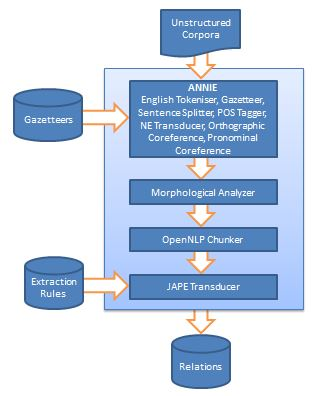
\includegraphics{archidesign1.jpg}      %-- include image file named as "sinag1.eps" 
   \caption{Architectural Design}
    \label{fig:archidesign}
\end{figure}

Each children's story text from the \textit{unstructured corpora} is opened in GATE by creating a GATE Document. Once the GATE documents are created, the next step is to create a GATE Corpus and add the documents. First, the GATE application resets the input of any previous annotations. This applies only if the input has already been annotated before passing through GATE. After cleaning, the input is parsed into tokens. The input was then  split into sentences and each token was annotated with their respective part-of-speech tags. After that, named-entities from the defined gazetteers were annotated. Then, pronouns are matched with the named-entities they are referring to in the text. 

Then, each token are processed to identify their lemmas, affixes and chunks. Lastly, the input text is ran through a transducer. This will finally identify all the target relations and create the appropriate annotations for each.

The output of the GATE tool is an annotated version of the story that also contain the extracted target relations.

\subsubsection{Resolving Story-specific Named Entities}
\label{sec:gazetteer}

In this implementation, a gazetteer resource was used to identify named entities in the input texts. However, the predefined lists does not cover some of the named entities in the children's story corpora. Such include characters, locations and roles. For example, in the \textit{Winnie the Pooh} set of stories, \textit{Pooh}, \textit{Piglet} and \textit{Tigger}, among others, are not included. Thus, additional lists are needed. Aside from the named entities found in stories, gazetteers are also created for indicators, world states and emotions, among others. These will be used by the transducer in its annotation patterns. A total of 20 new gazetteers were created for this study. Shown in Table \ref{tab:newgazetteersind} are the gazetteers created for indicators.

\begin{table}[H]   %t means place on top, replace with b if you want to place at the bottom
\centering
\caption{New Gazetteers (Indicators)} \vspace{0.25em}
\begin{tabular}{|p{5cm}|p{5cm}|} \hline
\textbf{File Name} & \textbf{Description} \\ \hline
isaindicator.lst			& IsA Indicators \\ \hline
partofindicator.lst			& PartOf Indicators \\ \hline
madeofindicator.lst			& MadeOf Indicators \\ \hline
oftennearindicator.lst		& OftenNear Indicators \\ \hline
capableofindicator.lst		& CapableOf Indicators \\ \hline
locationofindicator.lst		& LocationOf Indicators \\ \hline
usedforindicator.lst		& UsedFor Indicators \\ \hline
ownsindicator.lst 			& Owns Indicators \\ \hline
motivationindicator.lst		& Motivation Indicators \\ \hline
goalindicator.lst			& Goal Indicators \\ \hline
causeindicator.lst			& Cause Indicators \\ \hline
effectindicator.lst			& Effect Indicators \\ \hline
\end{tabular}
\label{tab:newgazetteersind}
\end{table}

Table \ref{tab:newgazetteersstory} shows the gazetteers created for the story characters, locations and objects. Others were added to assist in improving the extraction of target relations.

\begin{table}[H]   %t means place on top, replace with b if you want to place at the bottom
\centering
\caption{New Gazetteers (Miscellaneous)} \vspace{0.25em}
\begin{tabular}{|p{5cm}|p{5cm}|} \hline
\textbf{File Name} & \textbf{Description} \\ \hline
storyLoc.lst		& Story Locations \\ \hline
animal.lst			& Animals \\ \hline
bodypart.lst		& Body Parts \\ \hline
position.lst		& Spatial markers \\ \hline
object.lst			& Objects \\ \hline
character.lst		& Story Characters \\ \hline
emotion.lst			& Emotions \\ \hline
worldstate.lst 		& World States \\ \hline
\end{tabular}
\label{tab:newgazetteersstory}
\end{table}

\subsubsection{Recognizing Target Relations}
\label{sec:recogtarget}

In order to extract the target relations, a number of JAPE phases must be created to recognise and annotate them in the input texts. A total of 23 customized JAPE phases were created for this purpose. Shown in Table \ref{tab:newjaperel} are the new JAPE phases to recognize the target relations. 

\begin{table}[H]   %t means place on top, replace with b if you want to place at the bottom
\centering
\caption{New JAPE Phases (Target Relations)} \vspace{0.25em}
\begin{tabular}{|p{6cm}|p{5cm}|} \hline
\textbf{File Name} & \textbf{Description} \\ \hline
isARelation.jape					& IsA Phase \\ \hline
partOfRelation.jape					& PartOf Phase \\ \hline
madeOfRelation.jape					& MadeOf Phase \\ \hline
oftenNearRelation.jape				& OftenNear Phase \\ \hline
capableOfRelation.jape				& CapableOf Phase \\ \hline
locationOfRelation.jape				& LocationOf Phase \\ \hline
usedForRelation.jape				& UsedFor Phase \\ \hline
ownsRelation.jape 					& Owns Phase \\ \hline
effectOf.jape						& EffectOf Phase \\ \hline
effectOfIsState.jape				& EffectOfIsState Phase \\ \hline
eventForGoalEvent.jape				& EventForGoalEvent Phase \\ \hline
eventForGoalState.jape				& EventForGoalState Phase \\ \hline
happens.jape						& Happens Phase \\ \hline
hasRoleRelation.jape				& HasRole Phase \\ \hline
roleResponsibleForRelation.jape		& RoleResponsibleFor Phase \\ \hline
\end{tabular}
\label{tab:newjaperel}
\end{table}

Table \ref{tab:newjapemisc} shows the other JAPE phases that are prerequisites of the target relation JAPE phases. These tag the custom tags \textit{Event}, \textit{Goal}, \textit{GoalEvent}, \textit{GoalState}, \textit{Cause} and \textit{Effect}. \textit{Preprocessing1.jape} is responsible in identifying the named-entities added for the benefit of the existing corpora.

\begin{table}[H]   %t means place on top, replace with b if you want to place at the bottom
\centering
\caption{New JAPE Phases (Miscellaneous)} \vspace{0.25em}
\begin{tabular}{|p{5cm}|p{5cm}|} \hline
\textbf{File Name} & \textbf{Description} \\ \hline
cause.jape				& Identify causes \\ \hline
effect.jape				& Identify effects \\ \hline
event.jape				& Identify events \\ \hline
goal.jape				& Identify goals \\ \hline
goalEvent.jape			& Identify goal events \\ \hline
goalState.jape			& Identify goal states \\ \hline
preprocessing1.jape		& Identify named entities based on new gazetteers \\ \hline
\end{tabular}
\label{tab:newjapemisc}
\end{table}

The JAPE tool follows a sequence in performing the aforementioned phases. Shown below is the sequence in tagging the custom tags and extracting the target relations:

\begin{verse}
\itshape
preprocessing1 \\
goal \\
goalEvent\\
goalState\\
event\\
cause\\
effect\\
isARelation\\
propertyOfRelation\\
madeOfRelation\\
oftenNearRelation\\
locationOfRelation\\
capableOfRelation\\
usedForRelation\\
ownsRelation\\
hasRoleRelation\\
partOfRelation\\
roleResponsibleForRelation\\
eventForGoalEvent\\
eventForGoalState\\
effectOf\\
effectOfIsState\\
happens\\
\end{verse}

\textit{Preprocessing1.jape} is the first phase ran to identify and tag all the new named-entities found in the corpora. This is followed by the tagging of \textit{Event}, \textit{Goal}, \textit{GoalEvent}, \textit{GoalState}, \textit{Cause} and \textit{Effect}. These are prerequisites for the \textit{EventForGoalEvent}, \textit{EventForGoalState}, \textit{EffectOf},  \textit{EffectOfIsState} and \textit{Happens} phases. The rest of the phases were put in that sequence based on the order of their creation.

During each phase, the whole document is processed. This allows multiple relation types to be extracted from a single sentence.

\subsection{Post-Processing}
\label{sec:postprocessing}

After running the GATE tool to annotate the stories, all post-processing were done semi-automatically. Since the output of GATE is just the annotated version of the input corpus, the annotated stories were saved as XML from the GATE program. These XML files contain all annotations like \textit{Token} and \textit{Sentence}, among others.  The target relations were then extracted to a PBREL file. 

PBREL files are created for the purpose of this study. It contains all extracted target relations from a story. Aside from the relations and their corresponding concepts, the rules used to extract them are also included for debugging purposes. An excerpt from \textit{A wild weather day.pbrel} is shown below.

\begin{verse}
\itshape
UsedFor(snacks,eating) UsedForRelation3 \\
Owns(their,adventure) OwnsRelation3\\
Owns(Pierre,garden) OwnsRelation3\\
CapableOf(thunder,go) CapableOfRelation1\\
EffectOf(stopped blowing,stopped falling) EffectOf4\\
EffectOf(shook the clubhouse,looked out the window) EffectOf4\\
EffectOf(got really cold,turned into balls of ice) EffectOf4\\
\end{verse}

After creating PBREL files for each story, the extracted relations were then collated into a single CPBREL (Collated PBREL) file for each big group of stories (\emph{RAW} and \emph{MODIFIED}). Aside from collating, redundant relations were also removed. The final CPBREL files for the \emph{RAW} and \emph{MODIFIED} stories were used in the testing stage.







